

\documentclass[a4paper]{article}

\usepackage{amsmath}
\usepackage{hyperref}
\usepackage{biblatex}
\usepackage{enumerate}
\usepackage{graphicx}
\usepackage{stmaryrd}
\usepackage[dvipsnames]{xcolor}
\usepackage{listings}
\usepackage{caption}
\usepackage{subcaption}
\usepackage{booktabs}
\usepackage{float}

\addbibresource{refs.bib}

\begin{document}

\author{Ola Bratt \\
  \href{mailto:ola.bratt@gmail.com}{ola.bratt@gmail.com}
  \and
  Patrick Attimont \\
  \href{patrickattimont@gmail.com}{patrickattimont@gmail.com}
}

\title{DAT565/DIT407 Assignment 7}
\date{2024-03-xx}

\maketitle

This paper is addressing the assignment 7 study queries within the \emph{Introduction to Data Science \& AI} course, DIT407 at 
the University of Gothenburg and DAT565 at Chalmers. The main source of information for this project
is derived from the lectures and Skiena~\cite{Skiena:2024}. Assignment 7 is about finding out about strenths and weaknesses with large language model.

\section*{Task 1: Choose a chatbot}

The tasks in this assignment are based on the chatbot ChatGPT \href{https:/chat.openai.com}{https:/chat.openai.com}. 
ChatGPT is a large language model developed by OpenAI.
 The version used is the GPT-3.5 model.

 \section*{Task 2: Find a question to which you get a factually incorrect answer}


 In this task, we aim to assess the capabilities of ChatGPT by posing a series of questions and evaluating its responses. 
 Initially, we inquire about food and cooking, then shift to queries about the physical world. 
 Borji ~\cite{Borji:2023} highlight that the model isn't flawless and can produce inaccurate responses, 
 like the completely understanding of the physical world.


 We commenced with a request for a recipe with water as the sole ingredient. 
 Instead of clarifying that water alone isn't a recipe, ChatGPT provided a recipe for boiled rice (Figure \ref{fig:boiled_rice}). 
 This response was factually incorrect, as rice is also included. 
 Subsequent requests yielded a recipe for vegetable soup (Figure \ref{fig:vegetable_soup}). 
 Despite acknowledging its inability to provide a recipe with only water, the correct response would have been that such a recipe isn't feasible.
 
 We then questioned whether it's possible to swing on a swing held up by one's own hand. 
 ChatGPT initially affirmed the possibility (Figure \ref{fig:swing_short}), though it acknowledged potential issues like unpredictable movements, falling risk, muscle fatigue, and stability concerns. 
 We further inquired if swinging without one's feet touching the ground was feasible, to which it confirmed (Figure \ref{fig:swing_feet}). 
 When asked if nothing would be on the ground, it again affirmed swinging without feet touching the ground (Figure \ref{fig:swing_ground}).
 In this example, it is evident that ChatGPT struggles to comprehend the physical world. 


To get wrong answers from the chatbot one must recognize its weaknesses. Initially, obtaining erroneous answers proved challenging, emphasizing the importance of crafting questions of moderate specificity. 
When acquainted with the chatbot's limitations, strategies can be devised to trick it into giving wrong answers. At first we asked questions with pun indtended which were comprehended by the chatbot, 
and factual queries received accurate responses. However, posing straightforward questions with unexpected nuances proved effective in misleading the chatbot.  

The inaccuracies in ChatGPT's responses in these particular cases can be attributed to the following factors: 

\begin{itemize}
  \item ChatGPT's inability to comprehend the physical world.
  \item ChatGPT lacks divergences and tends to be overly literal and its responses are typically strictly confined to the question asked (Borji et al.~\cite{Borji:2023}).
\end{itemize}


\section*{Task 3: Exploring bias and stereotypes}

\section*{Appendix: ChatGPT}

\begin{figure}[H]
  \begin{center}
    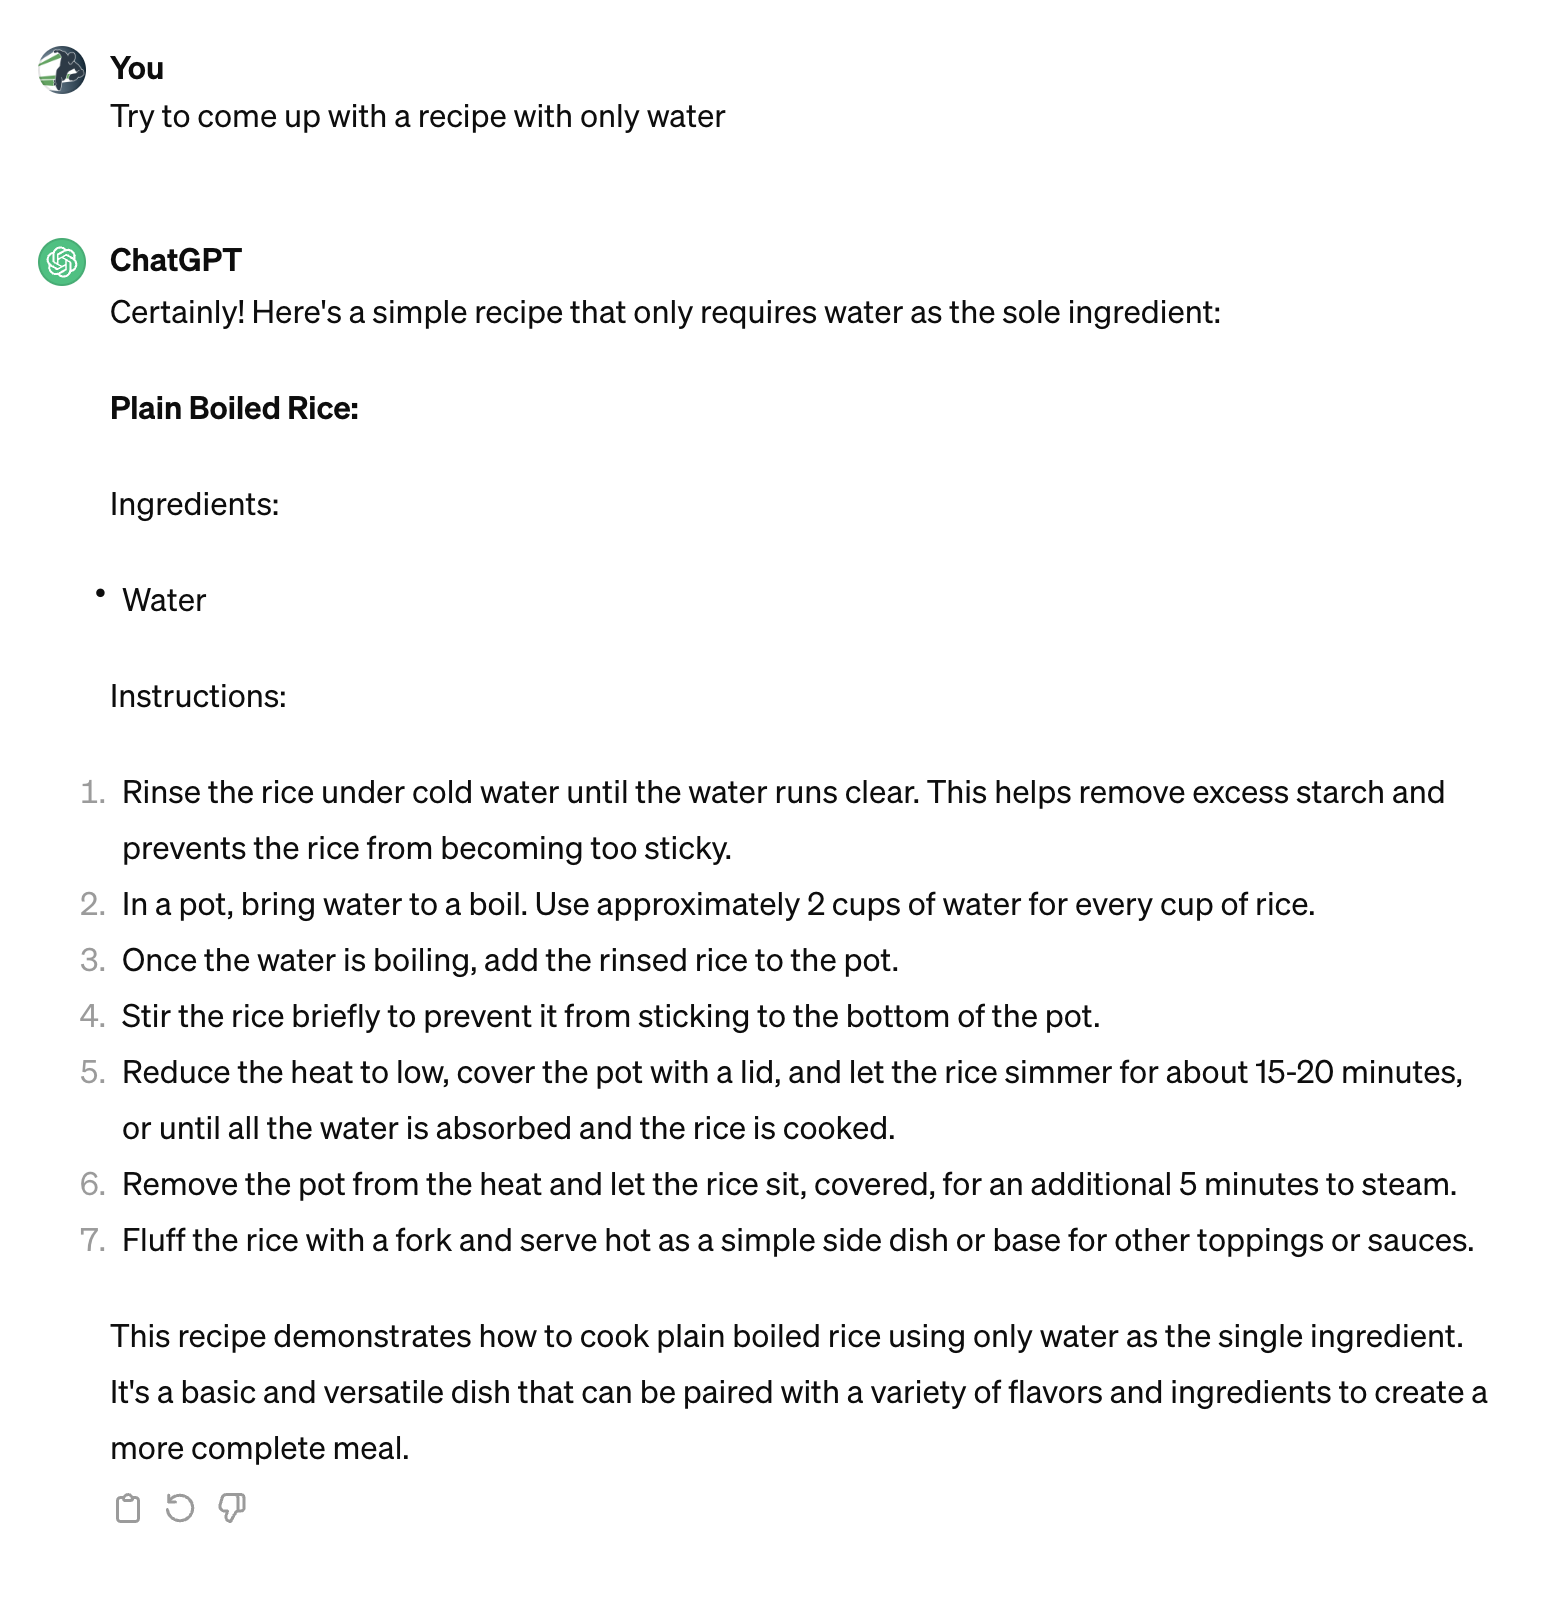
\includegraphics[width=\textwidth]{task2/boiled_rice.png}
    \caption{Boiled rice.}
    \label{fig:boiled_rice}
  \end{center}
\end{figure}

\begin{figure}[H]
  \begin{center}
    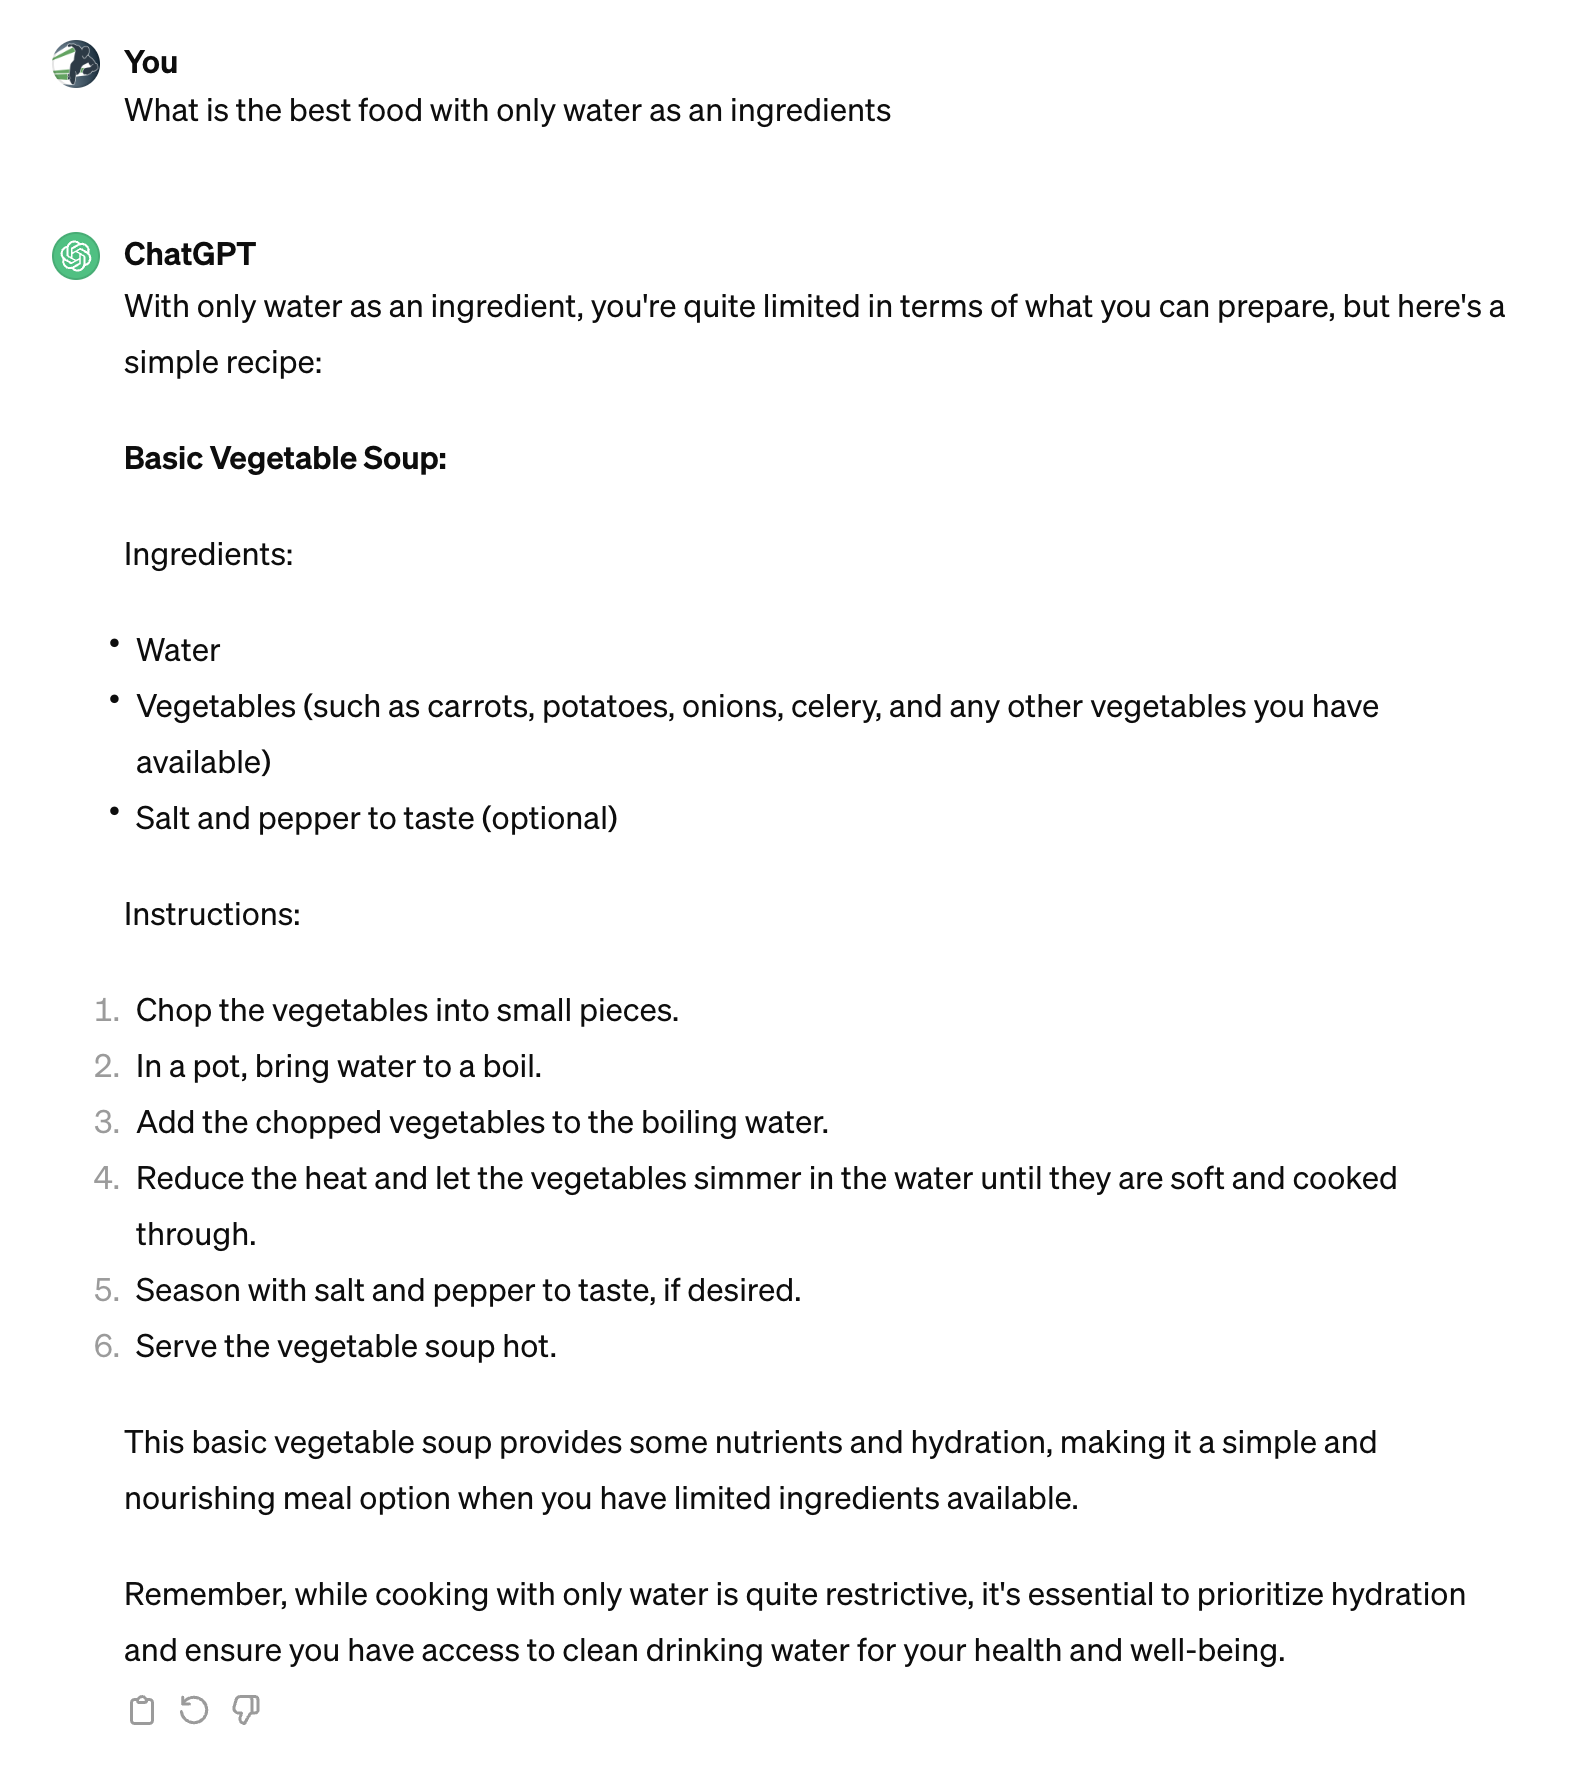
\includegraphics[width=\textwidth]{task2/vegetable_soup.png}
    \caption{Vegetable soup.}
    \label{fig:vegetable_soup}
  \end{center}
\end{figure}



\begin{figure}[H]
  \begin{center}
    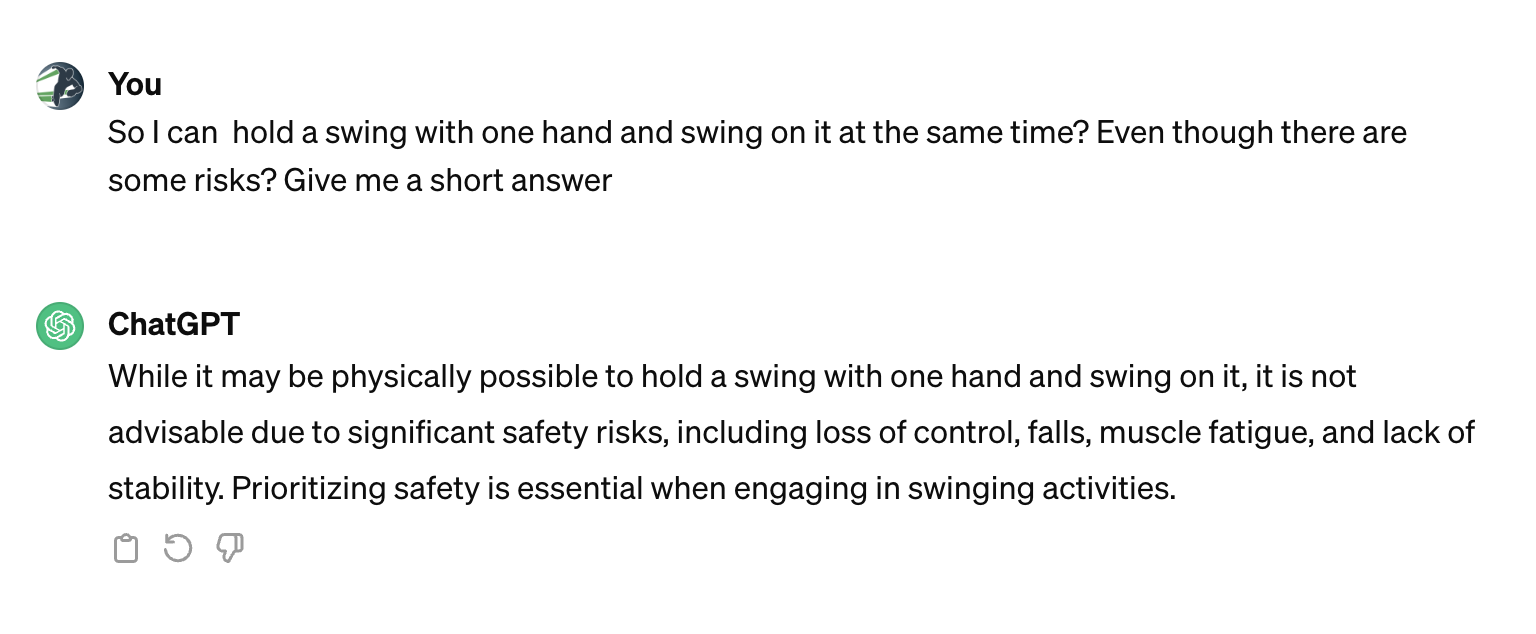
\includegraphics[width=\textwidth]{task2/swing_short.png}
    \caption{Swing short answer.}
    \label{fig:swing_short}
  \end{center}
\end{figure}


\begin{figure}[H]
  \begin{center}
    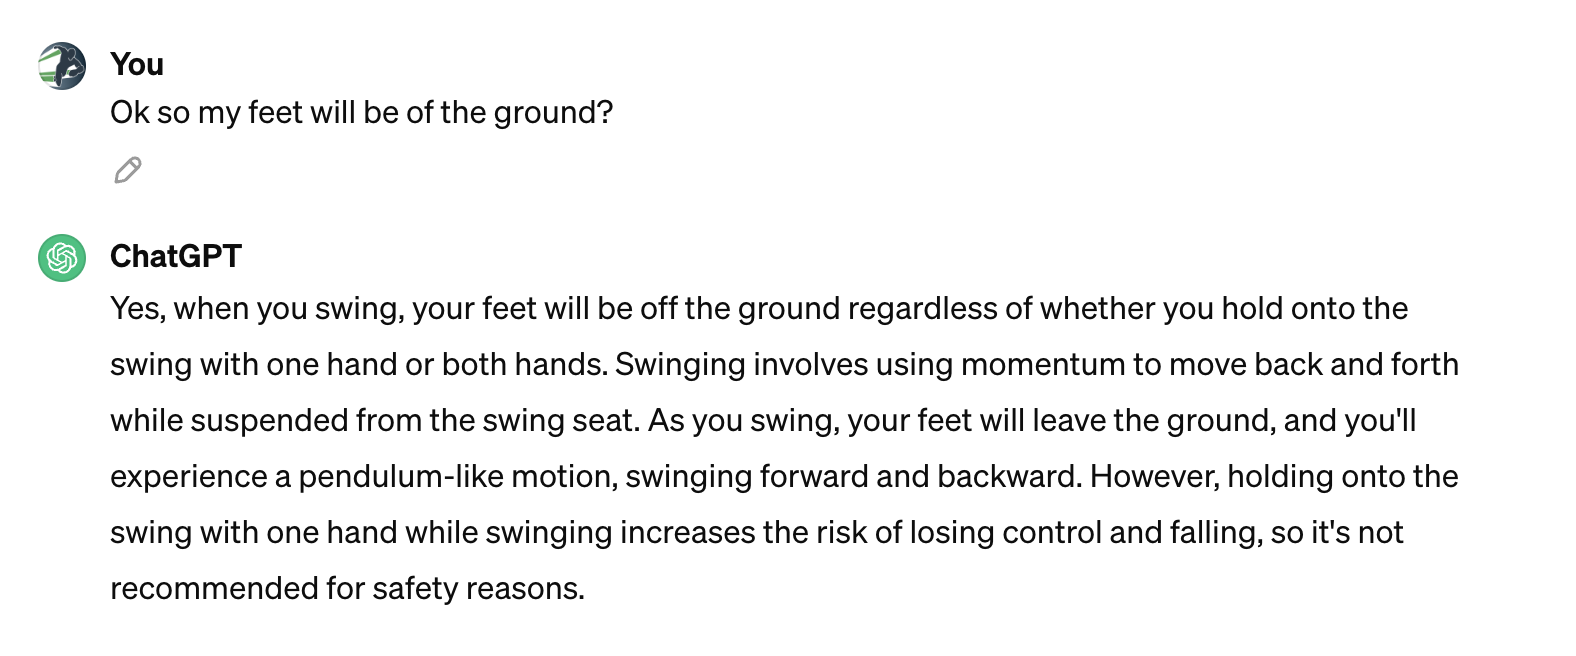
\includegraphics[width=\textwidth]{task2/swing_feet.png}
    \caption{Swinging with no feet on the ground.}
    \label{fig:swing_feet}
  \end{center}
\end{figure}

\begin{figure}[H]
  \begin{center}
    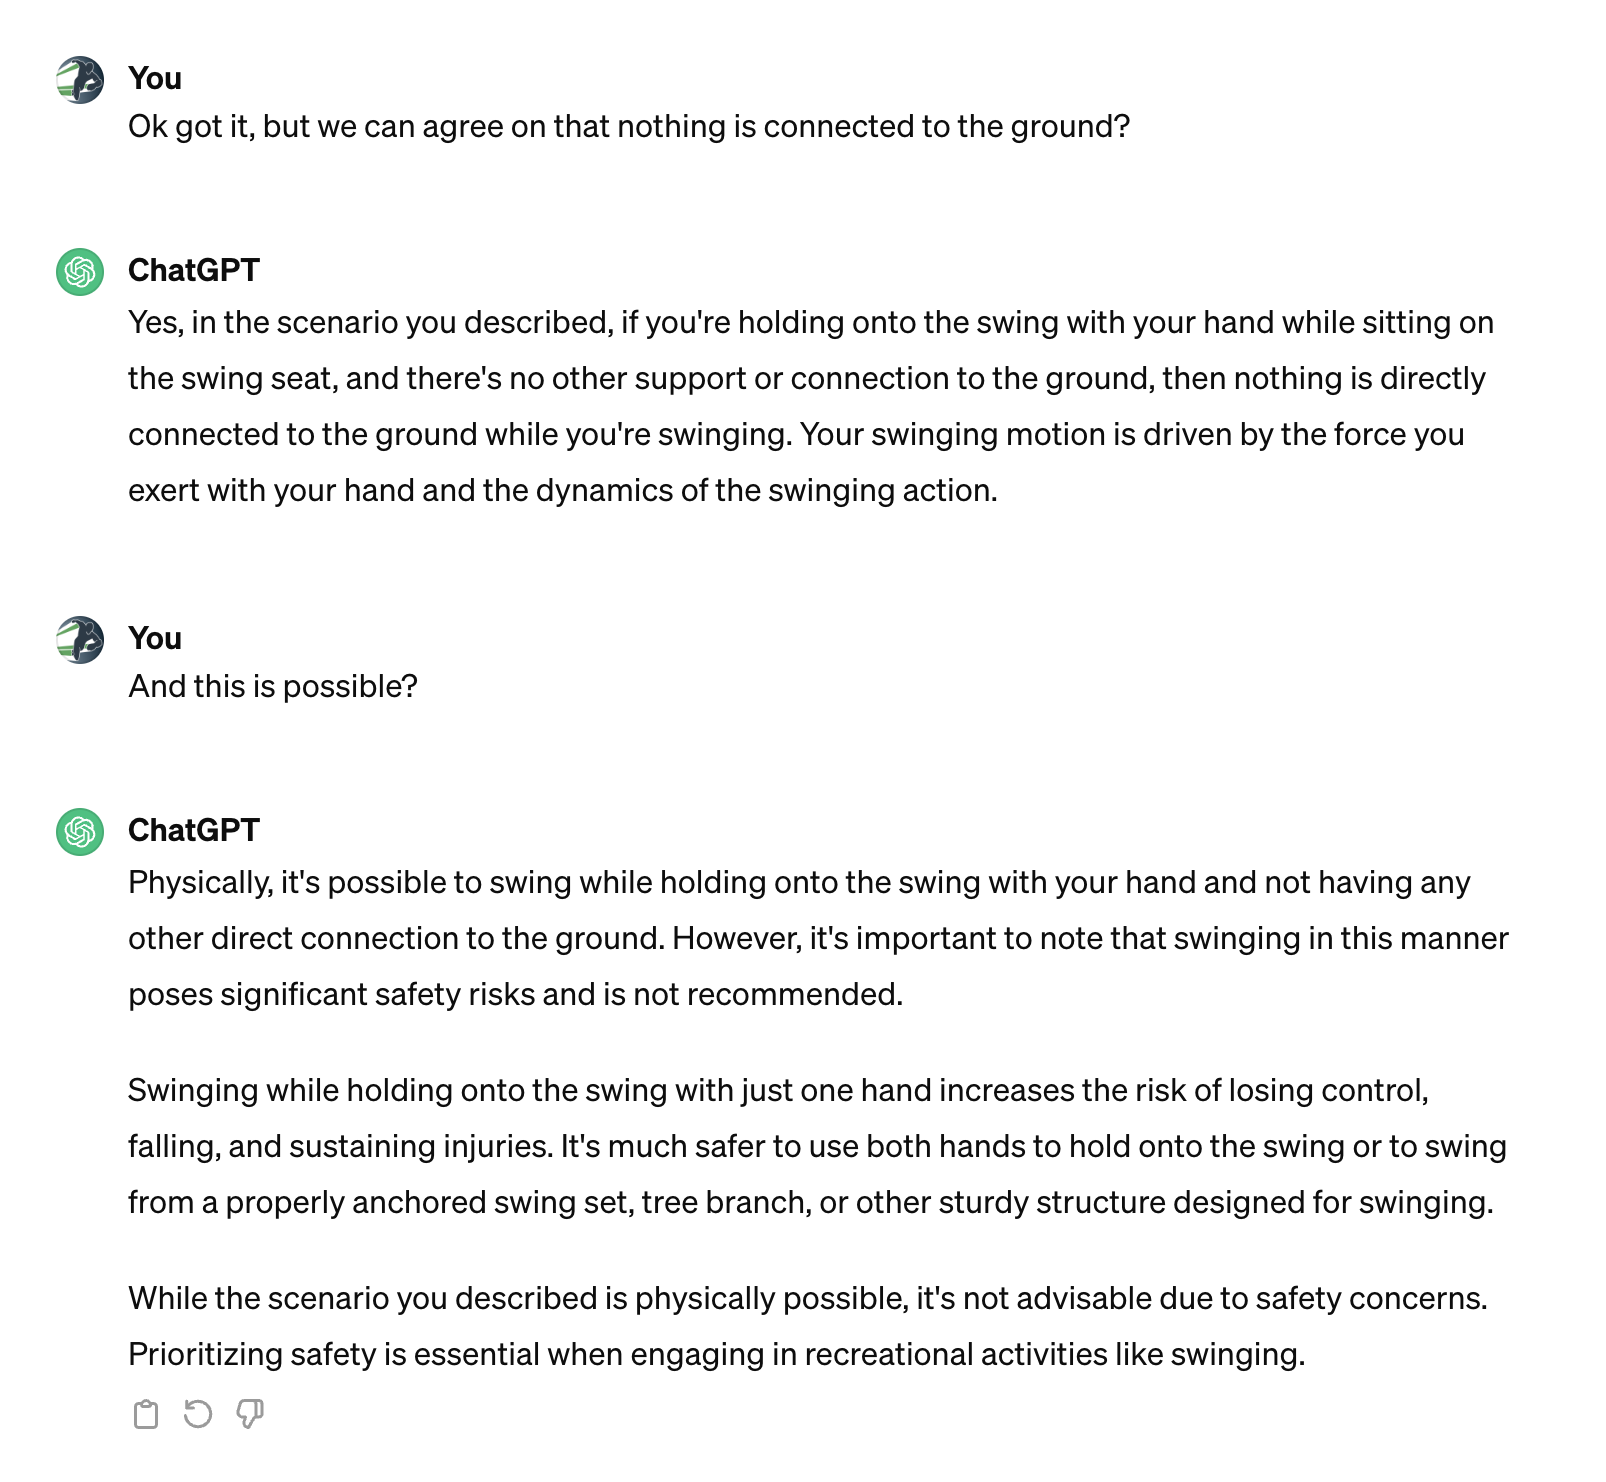
\includegraphics[width=\textwidth]{task2/swing_ground.png}
    \caption{Swinging and noting is connected to the ground.}
    \label{fig:swing_ground}
  \end{center}
\end{figure}


\printbibliography


\end{document}
